\documentclass[12pt]{article}
\usepackage{amsmath}
\usepackage{algorithm}
\usepackage[noend]{algpseudocode}
\usepackage{graphicx}
\usepackage{hyperref}
\usepackage{tikz,forest}
\usetikzlibrary{arrows.meta}
\usepackage{forest}
\usepackage{adjustbox}
\usepackage{skmath}
\usepackage{inputenc}
\usepackage{amsmath,amsthm,amssymb}
 \usepackage{tabu}
 \usepackage{graphicx}
\usepackage{wrapfig}
\graphicspath{ {images/} }
\usepackage{tcolorbox}
\newtheorem*{remark}{Remark}

\makeatletter
\def\BState{\State\hskip-\ALG@thistlm}
\makeatother

\forestset{
    .style={
        for tree={
            base=bottom,
            child anchor=north,
            align=center,
            s sep+=1cm,
    straight edge/.style={
        edge path={\noexpand\path[\forestoption{edge},thick,-{Latex}] 
        (!u.parent anchor) -- (.child anchor);}
    },
    if n children={0}
        {tier=word, draw, thick, rectangle}
        {draw, diamond, thick, aspect=2},
    if n=1{%
        edge path={\noexpand\path[\forestoption{edge},thick,-{Latex}] 
        (!u.parent anchor) -| (.child anchor) node[pos=.2, above] {Y};}
        }{
        edge path={\noexpand\path[\forestoption{edge},thick,-{Latex}] 
        (!u.parent anchor) -| (.child anchor) node[pos=.2, above] {N};}
        }
        }
    }
}


\begin{document}
\noindent

\noindent
{\large{Tackling Sequential Decision Problems}}\\

\noindent
What is sequential decision problems? Utility of the final result of the problem depends on a sequence of decisions of actions. These problems can be categorised into two types according to agents' abilities: \textbf{fully observable}, and \textbf{partially observable} problems. We will first look at problems with fully observable environments, then move on to partially observable environments.\\

\noindent
{\large{1. Markov Decision Process}}\\

Assumptions in MDP:
\begin{tcolorbox}
\begin{itemize}

\item \textsl{States}: set of all possible states that agents may end up in. 
\item \textsl{Actions}: set of all actions agents can choose to take.
\item \textsl{Transition model}: \textbf{assumes that we have a stochastic environment where the outcome of an action taken with a probability.} Therefore, we denote the output of the transition model as a probability: $P(s'| s, a)$, meaning the probability of being in $s'$ when action $a$ is taken in state $s$. $P(s'| s, a)$, thus, gives us a \textbf{3D table} with $s'$, $s$, and $a$ being its 3 dimensions.
			
\item \textsl{Rewards}: R(s) must be bounded, else gives an infinite value. 		
			
\item \textsl{Utility}: two types of utility functions are considered:  
\begin{itemize}
\item Discounted rewards: $U[s_0, s_1, s_2, ...] = R(s_0) + \gamma R(s_1) + (\gamma)^2 R(s_2) + ...$.
\item Additive rewards: $U[s_0, s_1, s_2, ...] = R(s_0) + R(s_1) + R(s_2) + ...$, a special case for discounted rewards when $\gamma  = 1$
\end{itemize}
 
\item \textsl{Policy}: a policy gives direction to an agent about which actions to take in a certain state. 

\end{itemize}
\end{tcolorbox}

\begin{remark}[Utility Function]
 We will utilise discounted rewards for all the problems by setting up $\gamma$ to a value between 1 and 0. This is because for problems with \textbf{infinite horizons}, where agent can go on forever in a game, the states sequence is infinite (which leads to an infinite utility value), but we still want to compare the utility of this infinite sequence of states with one another, thus, the utility value must be finite. Discounted rewards gives us exactly a finite utility value by apply a sum formula for a geometric series with $\gamma \leq 1$.  
\end{remark}

\begin{remark}[Policy]
One important point is that a fixed sequence of actions will never be a policy for stochastic environments. This is because in stochastic environment agents may end up in any state as the action given is probability based. Thus a good policy for MDP is the one which recommends agents which actions to take at any state at any episode. This leads us to a policy which is a state based, meaning gives agents guidance based on which state the agent is in, regardless of historical actions.
\end{remark}

\begin{remark}[Finite \& Infinite horizons]
MDP problems can be further classified as finite and infinite horizons. There is a difference in between these two concepts. For finite horizons, there is a fixed deadline for an agent to complete the game, thus with this deadline set differently, the agent may \textbf{balance rewards and risks} differently given how much time left, thus leads to different courses of actions (\textbf{nonstationary}) . However, for infinite horizons, we can think of it in this way: no matter how much time passed, we are always left with infinite amount of time, thus the agent does not have to change its plan of actions/policy (\textbf{stationary}) to achieve its optimal utility. The stationarity of policy assumes the stationarity of preference over state sequence as well. This means that if $[s_0, s_1, s_2 , ... ]$ is preferred over $[s_0, s_1', s_2', ...]$, then $[s_1, s_2, ...]$ is preferred over $[s_1', s_2', ...]$. The reason is that the same policy/optimal action at a certain state is the same at time $t+1$ and time $t$, therefore $[s_t, ...]$ should always preferred over $[s_t', ...]$.
\end{remark}

 To summarize: 
\begin{tcolorbox}
\textbf{Markovian Property}: the probability of reaching $s'$ from $s$ depends only on $s$ and not on the history of earlier states. 
\end{tcolorbox}

\begin{tcolorbox}
\textbf{Markov Decision Process}: a sequential decision problem for a fully observable, stochastic environment with a Markovian transition and additive rewards. 
\end{tcolorbox}

\pagebreak

\noindent
{\large{2. Looking For Optimal Policy}}\\

\noindent
To know which policy is optimal, we should know how to evaluate each policy and compare them. To evaluate policy, we take the expected utility generated by each policy and order them in their natural numerical order. Note that we use `expected' utility because sequences of actions generated by a policy corresponds to a probability. \\

\noindent
We denote a policy as $\pi$, and an optimal policy as $\pi^{*}$.  Thus, the expected utility of executing {$\pi$} starting from $s$ is: $U^{\pi}(s) = E[\sum_{t = 0}^{\infty} \gamma^t R(s_t) ]$. $\pi^{*}(s) = argmax U^{\pi}(s) = argmax \sum_{s'}^{} P(s' | s, a)U(s')$. We use $U(s)$ to denote the utility of executing an optimal policy from $s$.\\

There are two approaches for searching $\pi^{*}$, namely, value iteration and policy iteration.\\

\textbf{2.1 Value iteration}

Value iteration algorithm repeatedly updates the utility value of each state by executing Bellman update equation util an equilibrium (convergence) is reached where the utility values of stated are unchanged. \\

\begin{tcolorbox}

\textbf{Bellman equation} helps us to decide the utility value for a certain state when an optimal policy is deployed:\\
$U(s) = R(s) + \gamma max(a) \sum_{s'}^{} P(s' | s, a) U(s')$.\\

\textbf{Bellman update} updates the utility value for a state at time $t+1$ by consulting its neighbour's values at time $t$:\\
$U_{t+1} (s) \Leftarrow R(s) + \gamma max(a) \sum_{s'}^{} P(s' | s, a) U_t (s')$

\end{tcolorbox}

\begin{tcolorbox}

\textbf{Value iteration} will \textbf{converge} at some point for discounted rewards with $\gamma < 1$. This is because Bellman update $U_{t+1} \Leftarrow BU_{t}$ is a \textbf{contraction}: $||BU_{t+1} - BU_{t}|| \leq \gamma||U_{t+1} - U_{t}||$. \\

Thus, a fixed point would be reached: $||BU_{t} - BU||  = ||BU_{t} - U|| \leq \gamma ||U_{t-1} - U|| \leq  \gamma^2 ||U_{t-2} - U||  \leq ...  \leq \gamma^t ||U_{0} - U||$. (Note: $BU = U$ means $U$ reaching an equilibrium; $\gamma^t$: contract exponentially)

\end{tcolorbox}

\begin{tcolorbox}
Continue from $||BU_{t} - U||  \leq \gamma^t ||U_{0} - U||$. If we can accept a maximum error $\epsilon$ between $\pi^*$ and $\pi$, then $||BU_{t} - U||  \leq \gamma^t ||U_{0} - U|| \leq \epsilon $. From the geometric sequence of discounted rewards, we know that $||U_{0} - U|| \leq R_{max}/(1- \gamma)$, thus we have $\gamma^t \times R_{max}(1- \gamma) \leq \epsilon$, where $t$ is the number of Bellman update we should go through to find the our imperfect $\pi$ with error $\epsilon$ to $\pi^*$. Therefore, the termination condition for the value iteration algorithm is $||U_{t+1} - U{t}|| \leq \epsilon(1 - \gamma)/ \gamma$.
\end{tcolorbox}


\textbf{2.2 Policy iteration}

Policy iteration seems simpler than value iteration. We randomly initialize a policy and solve linear equations to get the utility value for each state. Then according to this state utility value to check whether any state action should be changed or not. If it is, we change the state action/policy according and re-calculate the utility values with the new policy. We iterate through this process util no state action is changed. Them we reach our equilibrium, and get $\pi^*$. \\

\begin{tcolorbox}
\textbf{Policy evaluation}: given a policy $\pi$, construct the state utility function according to the actions given by the policy, and solve the $n$ linear equations with $n$ unknown state utility values: 
$U(s) = R(s) +  \gamma \sum_{s'}^{} P(s' | s, \pi(s)) U(s')$.\\

\textbf{Policy improvement}: using one step look ahead (i.e. check whether the action is the optimal action by using the neighbour state utility values) to calculate a new policy based on the immediate (one step) neighbours' state utility value.
\end{tcolorbox}

\begin{remark}[Linear Equation]
Notice that the equations in policy iteration are \textbf{linear}. This is because given the policy, the utility value of each state can be calculated. There is no \textbf{max operator}, which is unlike value iteration where we do not know the policy thus need to use max operator to find the policy. For $n$ states, policy iteration evaluation can solve it in $O(n^3)$. 
\end{remark}

\begin{remark}[Approximation]
\textbf{Modified policy iteration} is used to iteration $k$ times instead of to convergence. \textbf{Asynchronous policy iteration} is to speed up the algorithm by executing iteration improvement and iteration evaluation for a subset of states. 
\end{remark}

\noindent
{\large{3. Online Search}}\\
Why do we need online search? because of the curse of dimensionality. For $n$ binary state variables, we have $2^n$ states to look at in both value and policy iteration. One way to handle this dimensionality (too many states) is to utilize \textbf{online search with sampling}.

\begin{tcolorbox}
At every step, if the state \textbf{does not have a policy to choose an action}, construct a search tree with the root node as the current state to decide the optimal action to take at the current state:
\begin{itemize}
\item Fix the depth of the search tree as $D$
\item $|A|$: the number of action nodes 
\item $|S|$: the number of observation nodes / chance nodes which gives the number of next state we can transition to 
\item Tree size: $A^D S^D$
\end{itemize}

\textsl{Value of the root}: initialize utility values/reward at the leaf nodes, walk way back. At \textbf{chance node}, compute the \textbf{expected utility}. At \textbf{action node}, take the \textbf{maximum} from the children. \\

\textsl{Conclusion}: the above does not solve the curse of dimensionality but makes the situation worse: the search space increases from $S$ to $A^D S^D$.\\

\textsl{Solution:} \textbf{sparse sampling}, sample $k$ states at the observation nodes, thus the search space size is reduced to $A^D k^D$, where $k$ does not depend on state space size $|S|$, but how accurate we want our approximation to be (same as $D$).\\

\textsl{Summary}: sparse sampling solves the curse of dimensionality, but not the curse of history, exponential with the search depth $D$. 

\end{tcolorbox}

\noindent
\textbf{3.1 Monte Carlo Tree Search}

MCTS is a form of online search because it corporates online search algorithm in its procedure. Its application extends beyond games, and MCTS can theoretically be applied to any domain that can be described in terms of \{state, action\} pairs and simulation used to forecast outcomes.

\begin{tcolorbox}
Basic algorithm: \\
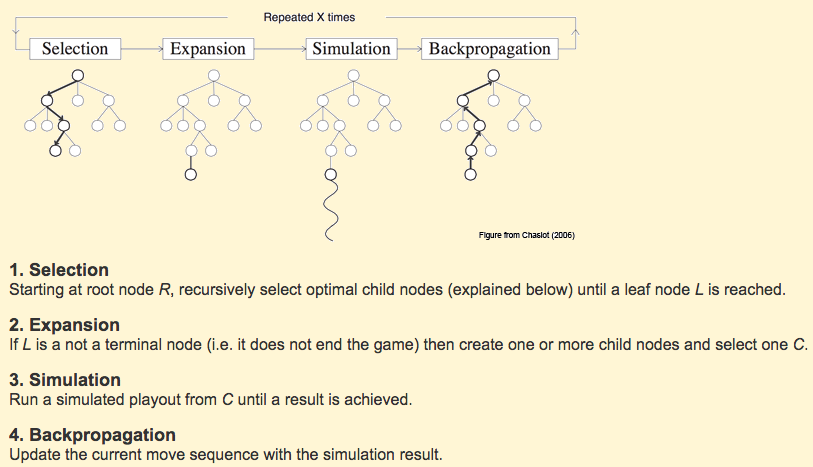
\includegraphics[scale=0.45]{MCTSalgo}

\begin{itemize}
\item Each node must contain two important pieces of information:

1. an estimated value based on simulation results\\
2. the number of times it has been visited


\item In its simplest and most memory efficient implementation, MCTS will add one child node per iteration. Note, however, that it may be beneficial to add more than one child node per iteration depending on the application.
\item Node selection during tree descent is achieved by choosing the node that maximises the \textbf{Upper Confidence Bounds (UCB)} formula:\\

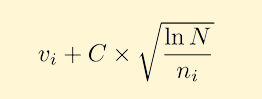
\includegraphics[scale=0.4]{UCB}      \textsl{exploitation term + exploration term}\\

where $v_i$ is the estimated value/average return of the node, $n_i$ is the number of the times the node has been visited and $N$ is the total number of times that its parent has been visited. $C$ is a tunable bias parameter.

\end{itemize}
\end{tcolorbox}

\begin{remark}[Anytime Policy]
MCTS deploys an \textbf{anytime policy}: when time is up, use the action that looks the best at the root at that time.
\end{remark}

\begin{remark}[Exploitation vs Exploration]
The UCB formula balances the exploitation of known rewards with the exploration of relatively unvisited nodes to encourage their exercise. Reward estimates are based on random simulations, so nodes must be visited a number of times before these estimates become reliable; MCTS estimates will typically be unreliable at the start of a search but converge to more reliable estimates given sufficient time and perfect estimates given infinite time.
\end{remark}

\begin{remark}[Benefits] 
Advantages of using MCTS:
\begin{itemize}
\item \textsl{Aheuristic}: MCTS does not require any strategic or tactical knowledge about the given domain to make reasonable decisions. The algorithm can function effectively with no knowledge of a game apart from its legal moves and end conditions; this means that a single MCTS implementation can be reused for a number of games with little modification, and makes MCTS a potential boon for general game playing.

\item \textsl{Asymmetric}: MCTS performs asymmetric tree growth that adapts to the topology of the search space. The algorithm visits more interesting nodes more often, and focusses its search time in more relevant parts of the tree. (Trade off between exploration and exploitation).
\end{itemize}
\end{remark}

\begin{remark}[Example]
A worked example of MCTS:  \\
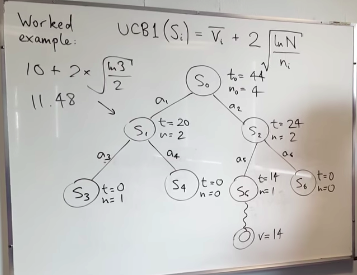
\includegraphics[scale=0.7]{UCBeg}

\end{remark}

\noindent
\textbf{3.1.1 Monte Carlo Tree Search With MDP}\\
By applying MDP in MCTS, we are adding observation nodes/chance nodes into the search tree. Agents make actions at the action nodes, and environment selects a next state with certain probability distribution at the observation nodes. Thus, action $a$ is selected by balancing the exploration and exploitation. 
\begin{tcolorbox}
\begin{itemize}
\item $r_t(n)$: the return value of $t_{th}$ trial at node $n$ with state $s$ and next node $n'$ is $R(s) + \gamma r_t(n')$, so $r_t(n)$ = $R(s) + \gamma r_t(n')$
\item $\overline Q(n, a)$: Q-function/action-value function, the average return of all the trails at node $n$ and action $a$
\item $\overline V(n)$: the estimated value at node n is the average return at node n over all the trials, thus $\overline V(n)$ = $max \overline Q(n, a)$ wrt action $a$
\end{itemize}
\end{tcolorbox}

\noindent
\textbf{3.2 Upper Confidence Tree}\\
UCT is built with MCTS, with the following functions to select actions at node $n$:\\
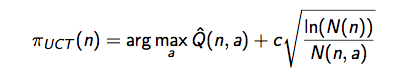
\includegraphics[scale=0.7]{UCT}\\
UCT will eventually converge to the optimal policy with enough trials. The worst case can be very bad: $\Omega(exp(exp( ... exp(1) ...)))$ with $D-1$ times $exp$.\\

\noindent
\textbf{3.3 Alpha Go}\\
Alpha Go is a zero-sum game instead of a MDP, but it utilizes MCTS and deep neural network.
\begin{tcolorbox}
\begin{itemize}
\item Deep neural network with two heads: 
\begin{itemize}
\item Value head: output a real value estimate of the value function
\item Policy head: output a vector where each component represents the probability that the policy will play the game
\end{itemize}
\end{itemize}
\end{tcolorbox}

\begin{tcolorbox}
\begin{itemize}
\item MCTS: is used to select actions
\begin{itemize}
\item Variant of UCT that exploits policy head output of neural network $P(s, a)$.\\
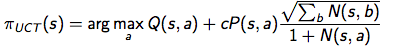
\includegraphics[scale=0.7]{go}
\item When the leaf node is reached, the value head of the neural network is used to estimate the state instead of doing a simulation/roll-out.
\end{itemize}

\item Since this is a zero-sum turn taking game instead of a MDP, the search alternates between selecting action that maximizes when it is first player's turn and action that minimizes (multiply estimate by $-1$ then maximize) for second player's turn. At termination, reward $+1$ for first player win and $-1$ for second player win.
\end{itemize}
\end{tcolorbox}

\underline{\textsl{Additional Notes:}}

\pagebreak 
\noindent
{\large{Decision Making Under Uncertainty}}\\

\noindent
What makes \textbf{planning} hard is that we have to consider utilities of \textbf{long sequences of actions} to reach a certain goal. \textbf{Uncertainty} makes decision making for each decision hard. We will use \textbf{decision theory} to make rational decisions under uncertainty base on \textbf{preferences} over the underlying outcome states. Therefore, it is necessary for us to first look at what is decision theory. \\

\noindent
{\large{Decision Theory}}\\
\begin{tcolorbox}
Decision theory is a calculus for decision-making under uncertainty. To utilize this theory, we will make the following assumptions:\\
\begin{itemize}
\item A set of possible \textbf{outcomes} in the domain of interest
\item  A set of \textbf{preferences} (of the agent) over the possible outcomes
\item The \textbf{probabilities} of different outcomes actually happening in various situations
\end{itemize}
Then, we will model uncertain outcomes as lotteries, e.g. $[p, A; 1-p, B]$. To see how to make decision among different lotteries, we need to determine the expected utility of each lottery, and choose the \textbf{maximum} among them. 
\end{tcolorbox}

\begin{tcolorbox}
\textbf{Principle of maximum expected utility (MEU)}: a rational agent should choose the action that maximizes its expected utility. 
\begin{itemize}
\item $P(RESULT(a) = s' | a, e )$: the probability of outcome $s'$ given that action $a$ and evidence $e$
\item $U(s)$: utility function assigning a number to indicate desirability of state $s$
\item $EU(a|e) = \sum_{s'}^{} P(RESULT(a) = s' | a, e)U(s')$: the expected utility of action $a$ given evidence $e$.
\end{itemize}
\end{tcolorbox}

\begin{tcolorbox}
MEU is based on the \textbf{utility theory}, which contains the following \textbf{six axioms}. If your agent's preferences meet the requirements in the axioms, then decision theory/MEU will tell you how to make your decisions. If you disagree with the axioms, then you have to find another way of choosing actions.\\

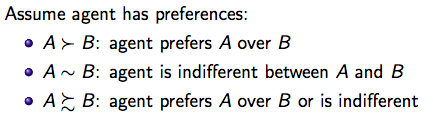
\includegraphics[scale=0.5]{p1}\\

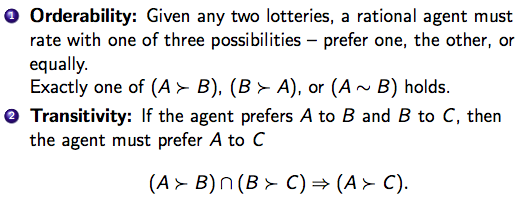
\includegraphics[scale=0.5]{p2}\\
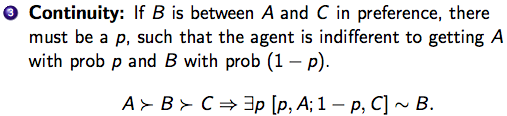
\includegraphics[scale=0.5]{p3}\\

\begin{itemize}
\item  In the first lottery, you get your best outcome, A, with probability p, and your worst outcome, C, with probability 1-p. 
\item In the second lottery, you get the outcome, B, with \underline{certainty}.
\item So, the idea is that, by adjusting p, you can make these lotteries \underline{equivalently attractive}, for any combination of A, B, and C.
\end{itemize}

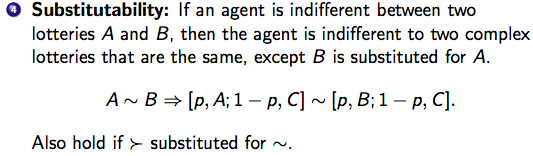
\includegraphics[scale=0.5]{p4}\\
\begin{itemize}
\item  If you prefer A to B, then given two lotteries that are \underline{exactly the same}, except that one has A in a particular position and the other has B, you should prefer the lottery that contains A.
\end{itemize}
\end{tcolorbox}

\begin{tcolorbox}
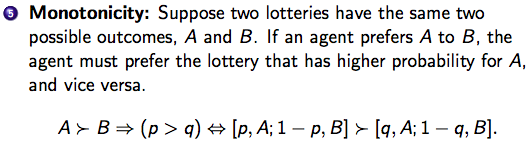
\includegraphics[scale=0.5]{p5}\\

\begin{itemize}
\item Monotonicity says that if you prefer A to B, and if p is greater than q, then you should prefer a lottery that gives A over B with higher probability.
\end{itemize}

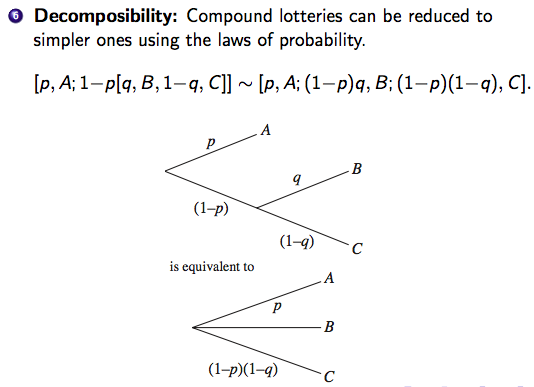
\includegraphics[scale=0.5]{p6}\\
\begin{itemize}
\item It, in some sense, defines \underline{compound} lotteries.
\item  It says that a two-stage lottery, where in the first
stage you get A with probability p, and in the second stage you get B
withprobability q and C with probability 1-q is equivalent to a single-stage
lottery with three possible outcomes: A with probability p, B with probability
(1-p)*q, and C with probability (1-p)*(1-q).
\end{itemize}
\end{tcolorbox}

\begin{tcolorbox}
Utility theory is really the axioms about preferences, nothing about the utility function ($U(s)$). However, from the utility theory,  the following consequences about $U(s)$ can be derived:

\begin{itemize}
\item \textbf{Existence of Utility Function}: There exists a realvalued
function U such that if you prefer A to B, then U(A) is greater than
U(B), and if you prefer A and B equally, then U(A) is equal to U(B). \\

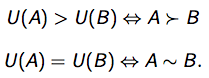
\includegraphics[scale=0.5]{p7}
\begin{itemize}
\item Basically, this says that all possible outcomes can be mapped onto \underline{a single
utility scale}, and we can work directly with utilities rather than collections of
preferences.
\end{itemize}

\item \textbf{Expected Utility of a Lottery}: The utility of a lottery is the expected
utility of the outcomes. \\

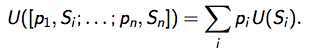
\includegraphics[scale=0.5]{p8}

\end{itemize}

An agent can act \textbf{rationally} only by choosing an action that \textbf{maximises the expected utility}.
An agent's behaviour does not change of the utility function is transformed an \textbf{affine transformation} $U'(s) = aU(s) +b$ with $a > 0$.\\

In a deterministic environment, only the axiom of orderability and transitivity are required. The other axioms all involves lotteries. 
\end{tcolorbox}

\pagebreak
\noindent
{\large{Utility Assessment}}\\
\begin{tcolorbox}
\begin{itemize}
\item \textbf{Preference elicitation}: the process of presenting choices to agents and working out the utility function from observed responses.
\item Fixing utilities of two outcomes sufficient to establish scale, usually fix for worst outcome $u_{\bot}$ and best outcome $u_{\top}$. For \textbf{normalized utilities}, fix values are $u_{\bot} = 0$ and $u_{\top}= 1$.
\item We can \textbf{assess utility for prize S} by asking agent to choose between prize and a standard lottery $[p, u_{\top}; 1-p, u_{\bot}]$. By adjusting p until agent is indifferent between S and lottery, then we can get the utility value for price S.
\end{itemize}
\end{tcolorbox}

\noindent
{\large{Utility of Money}}\\

\begin{tcolorbox}
\textbf{Risk Averse}: \\

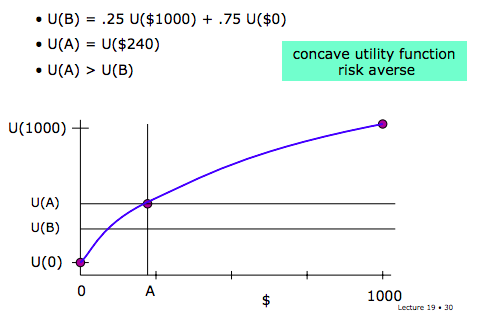
\includegraphics[scale=0.5]{p9}\\

\begin{itemize}
\item This describes a person who would in general prefers a smaller
amount of money for sure, rather than lotteries with a larger expected
amount of money (but not expected utility). Most people are risk averse in
this way.
\end{itemize}
\end{tcolorbox}
\begin{remark}
It's important to remember that decision theory applies in any case. It's not
necessary to have a utility curve of any particular shape (in fact, you could
even prefer less money to more!) in order for decision theory to apply to you.
You just have to agree to the 6 axioms.
\end{remark}

\begin{tcolorbox}
\textbf{Risk Neutral}:\\

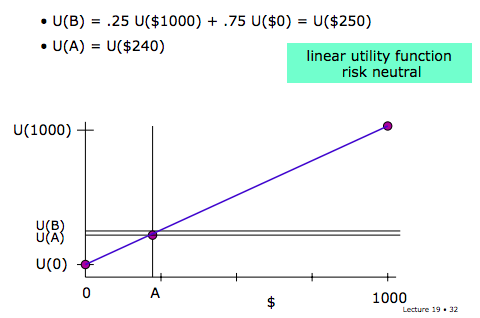
\includegraphics[scale=0.5]{p10}\\

\begin{itemize}
\item  If you are `risk neutral', then your utility
function over money is linear. In that case, your expected utility for a lottery
is exactly proportional to the expected amount of money you'll make. So, in
our example, the utility of B would be exactly equal to the utility of \$250. And
so it would be greater than the utility of A, but not a lot.
\end{itemize}

\end{tcolorbox}


\begin{tcolorbox}
\textbf{Risk Seeking}:\\

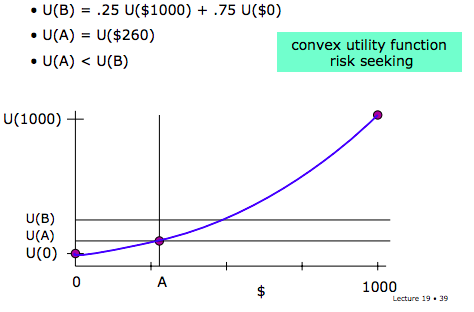
\includegraphics[scale=0.5]{p11}\\

\begin{itemize}
\item It's possible to argue that people play the lottery for a variety of reasons,
including the excitement of the game, etc. But here we've argued that there
are utility functions under which it's completely rational to play the lottery, for
monetary concerns alone. You could think of this utility function applying, in
particular, to people who are currently in very bad circumstances. For such
a person, the prospect of winning \$10,000 or more might be so dramatically
better than their current circumstances, that even though they're almost
certain to lose, it's worth \$1 to them to have a chance at a great outcome.
\end{itemize}

\textbf{Risk Seeking in Losses}\\

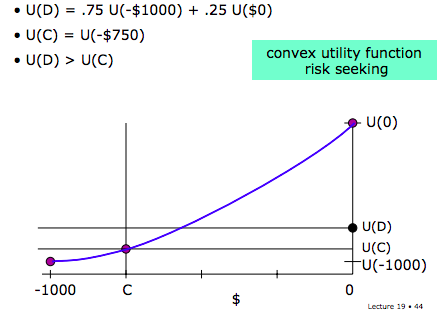
\includegraphics[scale=0.5]{p12}\\

\end{tcolorbox}

\begin{tcolorbox}
\begin{itemize}
\item In any real lottery, the expected amount of money you'll win is always less
than the price. 
\item  we can see that these preferences
imply a \textbf{convex utility function}, which induces risk seeking behavior. It is
generally found that people are risk seeking in the domain of losses. Or, at
least, in the domain of small losses.
\item An interesting case to consider here is that of \textbf{insurance}. You can think of
insurance as accepting a small guaranteed loss (the insurance premium)
rather than accepting a lottery (not risk seeking) in which, with a very small chance, a terrible
thing happens to you. So, perhaps, in the domain of large losses (in the case of insurance), people's
utility functions tend to change curvature and become concave again.
\end{itemize}
\end{tcolorbox}

\noindent
{\large{Optimizer's curse}}\\


\begin{tcolorbox}
As our model is the oversimplified version of the reality, we are really working with estimated expected utility value instead if the true expected utility value. This is mainly because, 1) we may not know enough about the reality; 2) the computation of the true expected utility is too difficult. Therefore, the real outcome is usually \textbf{worse} than our computation. This is because we are \textbf{choosing actions with the highest utility estimate}, obviously favouring the optimistic estimates, and this is \textbf{the source of the bias}. \\
\end{tcolorbox}

\begin{tcolorbox}
With \textbf{more choices} ($k$ indicated the number of choices in the following diagram), extremely \textbf{optimistic} estimates are \textbf{more} likely to arise, thus the greater the disappointment. It can even be the case that what appears to be the best choice may not be, if the variance in the utility estimate is high. \\

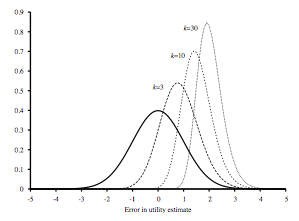
\includegraphics[scale=0.7]{p13}\\

We can \textbf{avoid the curse} by using an explicit probability model $P(\overline{EU} | EU)$ of the error in the utility estimates. Given this model and a prior $P(EU)$ on what we might reasonably expect the utility to be, we treat the utility estimate, once obtained, as evidence and compute the \textbf{posterior distribution for the utility} using \textbf{Bayes' rule}. 
\end{tcolorbox}

\noindent
{\large{Human irrationality}}
\begin{tcolorbox}
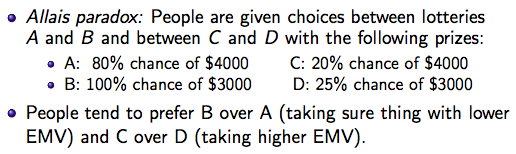
\includegraphics[scale=0.6]{p14}
\end{tcolorbox}

\begin{tcolorbox}
\begin{wrapfigure}{l}{0.5\textwidth}
    \centering
    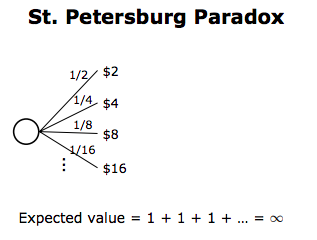
\includegraphics[width=0.45\textwidth]{p15}
\end{wrapfigure}
It was this paradox that drove Bernoulli to think about concave, risk averse,
utility curves, which you can use to show that although the game has an
infinite expected dollar value, it will only have a finite expected utility for a
risk averse person.
\end{tcolorbox}

\begin{tcolorbox}
\begin{itemize}
\item Certainty effect: people are strongly attracted to gains that are certain
\item Ambiguity aversion: prefer known probability to unknown ones
\item Framing effect: exact wording of choices have big impact on choices
\item Anchoring effect: people prefer to make relate utility judgements to absolute ones. They rely too much on initial information
\end{itemize}
\end{tcolorbox}

\noindent
{\large{Multiattribute Utility}}\\
1. Dominance
\begin{tcolorbox}
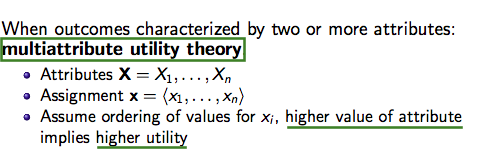
\includegraphics[scale=0.6]{p16}
\end{tcolorbox}


\begin{tcolorbox}
\begin{itemize}
\item \textbf{Strict dominance}: If an option is of lower value on all attributes than some other option, can be eliminated
\begin{itemize}
\item Example: \\
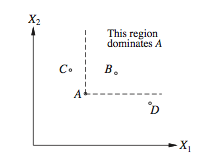
\includegraphics[scale=0.8]{p17}
\item When outcome \underline{uncertain}, can also eliminate A when all possible outcomes from B, D strictly dominates all possible outcomes for A
\end{itemize}

\item \textbf{Stochastic dominance}: a more useful generalization, can also eliminate an option if it is stochastically dominated on all attribute by another option\\
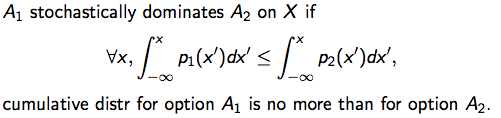
\includegraphics[width=0.9\textwidth]{p18}
\begin{itemize}
\item Expected utility of A1 at least as high as A2.
\end{itemize}

\begin{itemize}
\item Example: \\
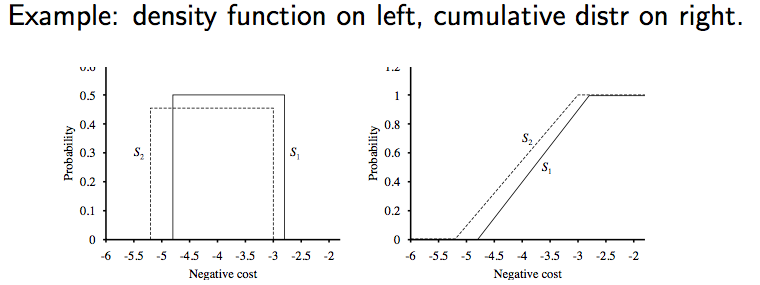
\includegraphics[scale=0.4]{p19}
\item $S_1$ dominates $S_2$
\end{itemize}

\end{itemize}
\end{tcolorbox}

2. Preference structure
\begin{tcolorbox}
Suppose we have $n$ attributes, each of which has $d$ distinct possible values. To specify the complete utility function $U(x_1, x_2, ..., x_n)$ we need \textbf{$d^n$} values in the \textbf{worst case}. This worst case corresponds to a situation in which the agent's preferences have no regularity at all. \textbf{Multi-attributes utility theory} is based on the supposition that the preferences of typical agents have much more structure than that. The \textbf{basic approach} is to \textbf{identify regularities} in the preference behaviour we would expect to see and to use what are called \textbf{representation theorem} to show that an agent with a certain kind of preference structure gas a utility function: $U(x_1, x_2, ..., x_n) = F[f_1(x_1), ..., f_n(x_n)]$, where $F$ is, we hope, a simple function such as addition. 
\begin{itemize}
\item \textbf{Preference without uncertainty}
\begin{itemize}
\item This is a deterministic case as there is no uncertainty
\item The basic regularity arises in deterministic preference structure is called \textbf{Preference independent (PI)}.
\item Preference independent: if $X_1$ is preference independent  of $X_2$ if 
 $(x_{1}, {x_{2}}^{0}) > (x_{1}^{'}, x_{2}^{0})$ implies that $(x_{1}, {x_{2}}) > (x_{1}^{'}, x_{2})$ for all $x_2$
 \begin{itemize}
 \item Example: Airport(Noise, Cost, Death), one may propose that Noise and Cost are preferentially independent of Death. 
 \end{itemize}
 
\end{itemize}
\end{itemize}
\end{tcolorbox}

\begin{tcolorbox}
\begin{itemize}
\item Preference without uncertainty (continue)
\begin{itemize}
\item \textbf{Mutual preferential independent (MPI)}: whereas each attribute may be important, it does not affect the way in which one trades off the other attributes against each other. 
\begin{itemize}
\item Airport(Noise, Cost, Death): (Noise, Cost) is preferentially independent of Death; (Cost, Death) is preferentially independent of Noise; (Noise, Death) s preferentially independent of Cost.
\end{itemize}
\item MPI implies \textbf{addictive preference function}:\\
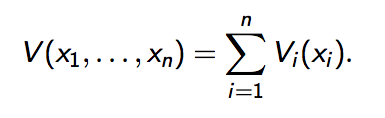
\includegraphics[scale=0.5]{p20}
 \begin{itemize}
 \item $V_i$ is a value function referring only to the attribute $X_i$
 \item For $n$ attributes, assessing an additive value function requires assessing n seperate one-dimensional value functions rather than one n-dimensional function, typically, this represents an \textbf{exponential reduction} in the number of preference experiments that are needed.
 \item Example: V(noise, cost, death) = -noise $\times 10^4$ - cost - death $\times 10^2$ 
 \end{itemize}
\item Additive preference function is often a \textbf{good approximation} even when MPI does not hold. This is espcially true when the violations of MPI occur in portions of the attributes. MPI is violated when attributes depends strongly on each other. 
\end{itemize}

\end{itemize}
\end{tcolorbox}

\begin{tcolorbox}
\begin{itemize}
\item Preferences with uncertainty
\begin{itemize}
\item When uncertainty is present, we need to consider the structure of preferences between lotteries and to understand the resulting properties of utility functions, rather than just value functions. 
\item \textbf{Utility independent}: A set of attributes X is utility independent of Y if preferences between lotteries on X are independent of values of Y.
\item \textbf{Mutually utility independent (MUI)}: A set of attributes is mutually utility independent if each of its subset is utility independent of the remainder.
\item MUI implies a \textbf{multiplicative utility function}: $U(x_1, x_2, x_3) = k_1U_1(x_1) + k_2U_2(x_2) + k_3U_3(x_3) + k_1k_2U_1(x_1)U_2(x_2) + k_1k_3U_1(x_1)U_3(x_3) + k_3k_2U_3(x_3)U_2(x_2) + k_1k_2k_3U_1(x_1)U_2(x_2)U_3(x_3)$
\begin{itemize}
\item The equation above contains just three single-attribute utility functions and three constants. In general, an \textbf{n-attribute problem} exhibiting MUI can be modelled using \textbf{n single-attribute utilities} and \textbf{n constant}. Each n single-attribute utility can be developed independently with the values under the attribute. 
\end{itemize}
\end{itemize}
\end{itemize}
\end{tcolorbox}

\pagebreak
\noindent
{\large{Decision Network}}

\begin{tcolorbox}
\textbf{Influence diagrams} or \textbf{decision networks} combine Bayesian networks with additional nodes to denote actions and utilities.\\

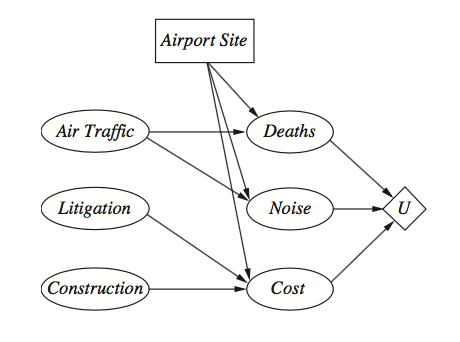
\includegraphics[scale=0.4]{p21}\\
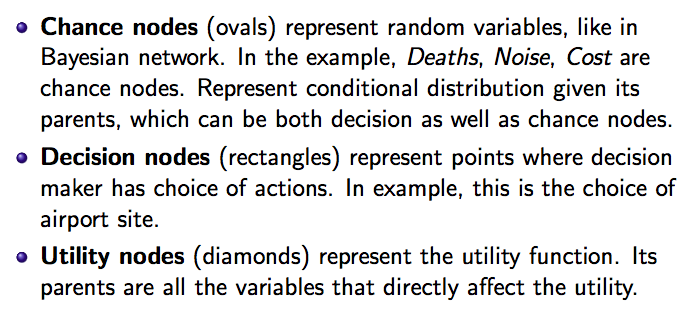
\includegraphics[scale=0.35]{p22}
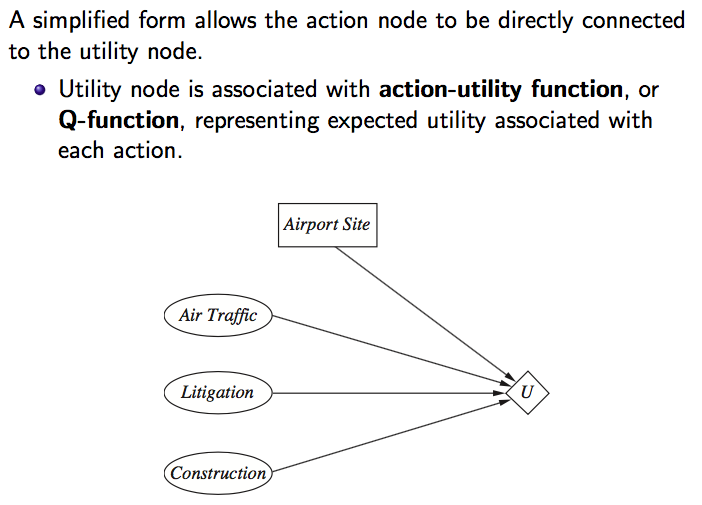
\includegraphics[scale=0.35]{p23}
\end{tcolorbox}

\begin{tcolorbox}
Evaluating Decision Networks\\

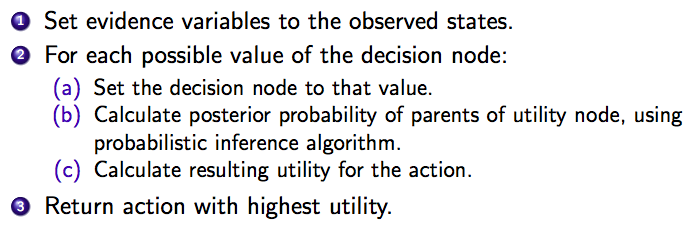
\includegraphics[scale=0.5]{p24}
\end{tcolorbox}


\noindent
{\large{Value of Information}}\\
Assume exact evidence can be obtained about variable $E_j$ (the evidence once observed, is certain), compute \textbf{value of perfect information}:
\begin{itemize}
\item  Given current evidence $e$, expected utility with current best action $\alpha$:\\
$EU(\alpha | e) =  \operatorname{arg\,max}_a \sum_{s'}^{} P(RESULT(\alpha) = s' | e, \alpha) U(s')$
\item Value of best new action after $E_j = e_j$ is obtained:\\
$EU(\alpha | e_i, e_j) = \operatorname{arg\,max}_a \sum_{s'}^{} P(RESULT(\alpha) = s' | e_i, e_j,  \alpha) U(s') $
\item Variable $E_j$ can take multiple values (for example, observed getting the land with gold, or not getting the land with gold), so must take the expected value:\\
$VPI(E_j) = \sum_{k}^{} P(e_{jk} | e) EU(\alpha_{jk} | e, e_{jk}) - EU(\alpha | e)$

\end{itemize}

\noindent
\textbf{Properties} of value of information: 
\begin{itemize}
\item Expected value of information in \textbf{non-negative}:\\
$\forall e, E_j, VPI_e(E_j) \geq 0$ 

\item VPI is \textbf{not additive}, but \textbf{order independent}:\\
 $VPI_e(E_j, E_k) = VPI_e(E_j) + VPI_{e, E_j}(E_k ) = VPI_e(E_k) + VPI_{e, E_k}(E_j )$
\end{itemize}



\end{document}